%%
%% This is file `esapub.tex',
%% generated with the docstrip utility.
%%
%% The original source files were:
%%
%% esapub.dtx  (with options: `manual')
%% ============================================
%% This is the manual describing the usage of
%%      esapub.cls
%% ============================================
%% Copyright 1999 Patrick W Daly
%% Max-Planck-Institut f\"ur Aeronomie
%% Max-Planck-Str. 2
%% D-37191 Katlenburg-Lindau
%% Germany
%% E-mail: daly@linmpi.mpg.de
%%
%% -------------------------------------------------
\documentclass[a4paper,twocolumn]{spaceDebrisC} % European paper
\pagestyle{empty}

% \bibliographystyle{alpha}
\bibliographystyle{apalike}

\usepackage{times}
\usepackage[numbers]{natbib}
\usepackage{graphicx}

\usepackage{bm} % for bold math
\usepackage{mathtools} % for \prescript
\newcommand{\vctr}[1]{\bm{#1}}
\newcommand{\unitv}[1]{\hat{\vctr{#1}}}
\newcommand{\preup}[1]{\prescript{#1}{}{}}
\newcommand{\rf}[1]{\mathcal{\MakeUppercase{#1}}}
\newcommand{\dcm}[1]{\left[\rf{#1}\right]}
\newcommand{\vrf}[2]{\preup{\rf{#1}}\vctr{#2}}
\newcommand{\mbar}[0]{\;\middle|\;}
\newcommand{\prf}[1]{\preup{\rf{#1}}}
\newcommand{\norm}[1]{\left\lVert#1\right\rVert}

\newcommand{\matcp}[1]{\left[#1 \times\right]}
\newcommand{\rthree}[0]{$\mathbb{R}^3$\:}
\newcommand{\sthree}[0]{$\mathbb{S}^3$\:}
\newcommand{\sothree}[0]{$SO_3$}
\newcommand{\pogslla}[0]{$32.900^\circ \textrm{ N}, -105.533^\circ \textrm{ W} \textrm{ }$}

\newcommand{\figbig}[0]{0.4\textwidth}
\newcommand{\figmed}[0]{0.4\textwidth}
\newcommand{\figsmall}[0]{0.3\textwidth}

\newcommand{\subfigmed}[0]{0.4\textwidth}
\newcommand{\subfigsm}[0]{0.29\textwidth}
\newcommand{\subfigbig}[0]{0.43\textwidth}

\DeclareMathOperator{\atantwo}{atan2}
\DeclareMathOperator{\fl}{floor}

\title{Optimal Light Curve Attitude Inversion with Measurement Noise: Two Case Studies}
\author{Liam Robinson}
\author{Carolin Frueh}
\affil{Purdue University, West Lafayette, United States, Email: \texttt{\{robin502, cfrueh\}$@$purdue.edu}}

\begin{document}

\keywords{Light curve inversion; Atitude estimation; Photometry; Inverse problems}

\maketitle

\begin{abstract}

Understanding the orientation and angular velocity state of active or passive human-made space objects is critical for many operations like long-term orbit propagation, aiding a mission, determining mission status, and active debris removal. Beyond low-Earth orbit, optical telescopes are used predominantly to track the space objects. Although this data is abundant, it is generally impossible to resolve even large satellites and rocket bodies in optical ground-based imagery due aperture size and atmospheric distortion. As a result, shape and orientation information is not available in any single image. But a measurement of the object's total brightness can still be obtained. Even if the object's shape and reflective properties are known, any given brightness measurement generally corresponds to infinitely many possible orientations. To constrain the solution space, the brightness can be tracked over time -- producing a sequence of measurements called a light curve. If the identity of the object is known, its attitude profile can be estimated from the light curve through a process known as light curve attitude inversion. Due to the natural and instrumental noise in the light curve, as well as symmetries in the observation geometry, there may be multiple attitude profiles which are equally likely to produce any given light curve.

\end{abstract}

\section{Introduction}

Knowledge of spacecraft orientation and angular velocity states is critical for many space situational awareness (SSA) tasks. Understanding the evolution of high area-to-mass ratio objects \cite{frueh2014} and decommissioned satellites \cite{rachman2023}, planning and executing active debris removal \cite{bonnal2013}, and recovering from mission anomalies \cite{umansky2023} all require attitude information.

[\textit{TODO: lit}]

In this work, we apply a light curve attitude inversion algorithm to real observations taken by the Purdue Optical Ground Station. Given an estimate of the shape and reflective properties of the object, our procedure searches the space of initial orientations, angular velocities, and inertia tensors to find initial conditions that produce light curves with low error compared to the observed values. Specifically, we estimate a full distribution for each candidate light curve and compute the likelihood of the observations being a sample from that distribution. To solve the optimization problem, we create a number of sampled candidate solutions, deterministically arranged throughout the solution space, and perform nonlinear optimization on each using the BFGS algorithm. This way, our optimization procedure reliably converges to all maximum likelihood estimates of the attitude state. Low-error minima are then clustered to identify families of nearby solutions with similar likelihood. The final output of our method is an array of the best solutions, ranked by their likelihood. Formulating the problem this way inherently accounts for the multiple classes of ambiguities resulting from the object and observation geometry, the physical constraints of torque-free rigid body motion, as well as the noise on the light curve.

To test the efficacy of this method, we perform attitude inversion on real observations gathered by the Purdue Optical Ground Station of an inactive GLONASS satellite and a rocket body. Solutions for the GLONASS case are analyzed to highlight the effect of observation geometry ambiguities, while the rocket body case highlights ambiguities introduced by the geometry of the object. Our noise model is validated against further real observations, confirming that all relevant noise sources have been accounted for and modeled accurately. We show that any significant lack of knowledge in the object shape or optical material properties causes the solution to rapidly degrade.


\section{Inversion Method}

\subsection{Objective Function}

Our inversion method is based on the global minimization of a maximum-likelihood loss function which computes the negative log-likelihood of the observed light curve $\vctr{S}$ being a sample from the normal distribution defined by the estimated light curve mean $\hat{\vctr{S}}$ and the estimated standard deviation at each $k$th timestep $\sigma_k$:

\begin{equation} \label{eq:nll_loss}
  f(\hat{\vctr{S}}, \vctr{S}) = \frac{1}{m}\sum_{k=1}^{m}\left[\ln\sigma_k + \frac{1}{2}\left(\frac{S_k - \hat{S}_k}{\sigma_k}\right)^2 \right].
 \end{equation}

In this work, the light curve and its standard deviation are always assumed to be expressed in a linear unit, e.g., analog-to-digital units (ADU) or irradiance.

\subsection{State Vector Definition and Dynamics}

The state vector $\vctr{x}$ we optimize to fit the observed light curve is the concatenation of the Modified Rodriguez Parameter (MRP) $\vctr{p} = [p_1, p_2, p_3]^T$, the principal body frame angular velocity $\vctr{\omega} = [\omega_1, \omega_2, \omega_3]$ in radians per second, and the ratios of the principal moments of inertia $J_y / J_x$ and $J_z / J_x$ where the full inertia tensor is $J = \mathrm{diag}\left([J_x, J_y, J_z]\right)$:

\begin{equation}
  \vctr{x} = \begin{bmatrix} 
  p_1 & p_2 & p_3 & \omega_1 & \omega_2 & \omega_3 & J_y / J_x & J_z / J_x
  \end{bmatrix}^T.
\end{equation}

The first six elements of the state vector are time varying with dynamics given by:

\begin{align}
  \vctr{\dot{p}} &= \frac{1}{4} \left[ \left(1 - \vctr{p} \cdot \vctr{p}\right) + 2\vctr{p} \times \vctr{\omega} + 2 \left(\vctr{\omega} \cdot \vctr{p} \right)\vctr{p} \right], \label{eq:mrp_kde} \\
  \vctr{\dot{\omega}} &= J^{-1} \left[ \left(J \vctr{\omega}\right) \times \vctr{\omega} + \vctr{M}\right]. \label{eq:rbtf_dynamics}
\end{align}

\section{Computing the Light Curve}

\subsection{Object Geometry Definition}

We choose to represent the surface geometry of space objects as a polyhedral mesh composed of a set of flat facets. Each $i$th face has $n_v \geq 3$ or more vertices $\left\{ v_{i,1}, v_{i,2}, v_{i,n_v} \right\}$ and an outward-pointing normal vector $\unitv{n}_i$. The total facet area is computed for an arbitrary planar polygon via:

\begin{equation} \label{eq:poly_area}
  A(P) = \sum_{j=0}^{k-3} \frac{\| \left( \vctr{v}_{j+1} - \vctr{v}_{j} \right) \times \left( \vctr{v}_{j+2} - \vctr{v}_{j} \right)\|_2}{2}.
 \end{equation} 
 
 In any particular illumination and observation condition, a fraction of the facet's area $\tilde{a}_i$ may be shadowed due to obstructing geometry before or after  light reaches the surface element. The remainder of the facet's area $\bar{a}_i$ is unshadowed and contributes to the total flux reaching the observer from the object, such that the total area of each facet is $a_i = \tilde{a}_i + \bar{a}_i$. The geometry for an individual facet is displayed in Figure \ref{fig:facet_geom}.

\begin{figure}[ht]
  \centering
  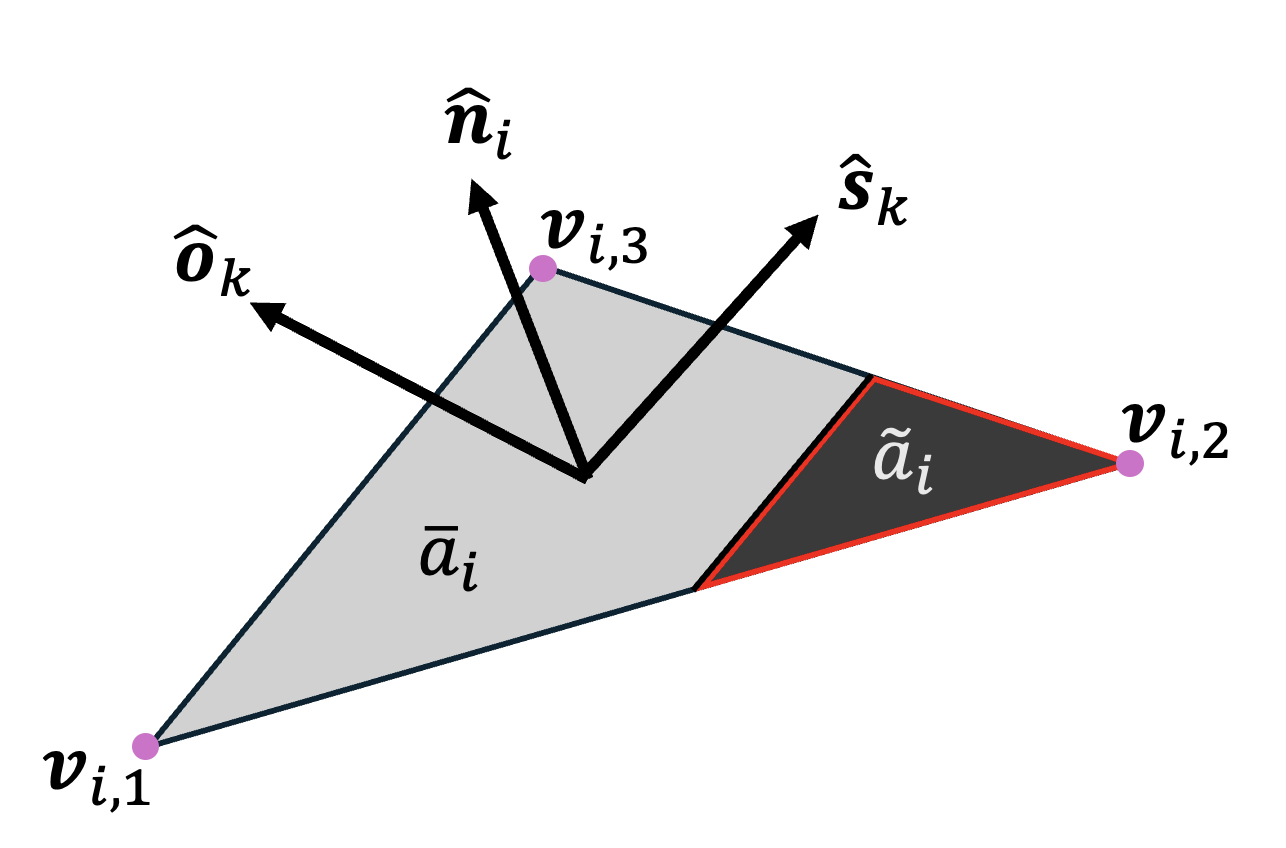
\includegraphics[width=\figmed]{obs_geom.png}
  \caption{Facet geometry including the observer direction $\unitv{o}$, Sun direction $\unitv{s}$, normal vector $\unitv{n}_i$, unshadowed area $\bar{a}_i$, shadowed area $\tilde{a}_i$, and counterclockwise vertex positions $\left\{ \vctr{v}_{i,1}, \vctr{v}_{i,2}, \vctr{v}_{i,3} \right\}$.}
  \label{fig:facet_geom}
\end{figure}

\subsection{Computing the Unshadowed Area}

The unshadowed area $\bar{a}$ may be computed in a number of ways. For convex objects, $\bar{a}=a$ as self-shadowing is impossible. For highly-nonconvex and detailed models composed of thousands of faces, $\bar{a}$ can be approximated on a pixel grid using shadow mapping \cite{robinson2022}. Self-shadowing can be solved semi-analytically for less detailed approximations of nonconvex objects by computing the mutual intersections of the polygons $P_k$ on other faces whose projections overlap with the face in question. Up to a maximum intersection depth $d$, the unshadowed area can be computed via:

\begin{equation} \label{eq:us_area}
  \bar{a} = a - \sum_{d=1}^{n} \sum_{K \in \text{comb}(n,d)} (-1)^{d+1} A\left(\bigcap\limits_{k \in K} P_k\right).
\end{equation}

As the objects we investigate in this work are well-approximated with relatively simple nonconvex meshes, we use the semi-analytic method to efficiently compute unshadowed areas via the Sutherland-Hodgeman algorithm \cite{sutherland1974} for each polygon intersection.

\subsection{Surface Reflectivity}

The bidirectional reflectance distribution function (BRDF) defines the amount of incident radiation from $\unitv{s}$ reflected per steradian in the observer's direction $\unitv{o}$. We choose the Blinn-Phong \cite{blinn1977} BRDF for this work as it is efficient to compute and satisfies the three main requirements for a physically-meaningful BRDF as it is nonnegative, energy-conserving, and reciprocal \cite{duvenhage2013}. The Blinn-Phong BRDF is parameterized by the coefficient of diffuse reflectivity $C_d$, the coefficient of specular reflectivity $C_s$, and the specular exponent $n>0$. The coefficients of reflectivity implicity satisfy $C_a + C_s + C_d = 1$ for energy conservation, where $C_a$ is the coefficient of absorption \cite{fan2020thesis}.

\begin{equation} \label{eq:brdf_blinn_phong}
  f_r(\unitv{s}, \unitv{o}) = \frac{C_d}{\pi} + \frac{n+2}{2\pi} \frac{C_s (\unitv{n} \cdot \unitv{h})^n}{4 (\unitv{n} \cdot \unitv{s})(\unitv{n} \cdot \unitv{o})}.
\end{equation}

Here, the halfway vector $\unitv{h}$ bisects the illumination and observation directions such that $\unitv{h} = \unitv{h} = (\unitv{s} + \unitv{o})/\norm{\unitv{s} + \unitv{o}}$ \cite{duvenhage2013}.

\subsection{The Light Curve}

Given the observer $\unitv{o}_k$ and illumination directions $\unitv{s}_k$ at the $k$th observation epoch in the body frame $\mathcal{B}$, as well as the BRDF $f_{r,i}$ for each $i$th surface of the object, the fraction of incident power reflected in the direction of the observer is \cite{fan2020thesis}:

\begin{equation} \label{eq:lc_norm}
  \begin{split} 
  f_p(\unitv{s}_k, \unitv{o}_k) = \sum_{i=1}^n\prf{B}[&\bar{a}_i(\unitv{s}_k, \unitv{o}_k) f_{r,i}(\unitv{s}_k, \unitv{o}_k) \\ \cdot &(\unitv{n}_i \cdot \unitv{s}_k) (\unitv{n}_i \cdot \unitv{o}_k)]. 
  \end{split} 
\end{equation}

The output of Equation \ref{eq:lc_norm} is a light curve, but as many of the noise characteristics of the signal are defined in image sensor's native unit of ADU, we convert the light curve into the same units via:

\begin{equation} \label{eq:general_bright}
  \begin{split} 
  \bar{S}_{\text{SO},k} = &f_p(\unitv{s}_k, \unitv{o}_k) \frac{A_\circ \Delta t_k f_\odot(\vctr{r})}{g R_\oplus^2 r_k^2} \\ \cdot &\int_{0}^{\infty}{P(\lambda)Q(\lambda)T_k(\lambda) I_\odot(\lambda) \left(\frac{\lambda}{hc}\right)}\,d\lambda. 
  \end{split}
\end{equation}

Here before the integral, $A_\circ$ is the unobstructed aperture area in square meters, $\Delta t_k$ is the exposure time in seconds, $f_\odot(\vctr{r})$ is the fraction of solar irradiance reaching the space object at position $\vctr{r}$ -- accounting for the Earth's shadow, $g$ is the sensor gain in ADU per photoelectron, $R_\oplus$ is the distance from the Sun to the space object in AU, $r_k$ is the distance from the observer to the space object in kilometers. Within the integral, we account for the telescope's passband filter $P(\lambda)$, the image sensor quantum efficiency $Q(\lambda)$, the atmospheric absorption spectrum $T_k(\lambda)$, the solar irradiance spectrum $I_\odot(\lambda)$, and the inverse energy of a photon with wavelength $\lambda$, $\lambda / hc$, where $h$ is Planck's constant in Joule-seconds, and $c$ is the speed of light in vacuum in meters per second. Taken together, the integral computes the fraction of the energy reflected from the object absorbed into the image sensor, while the the outer factor dimensionalizes the result to yield the mean total sensor response in ADU across all pixels due to the object's signal.

the variance a space object's light curve whose mean is determined by Equation \ref{eq:general_bright} is a combination of a number of relevant independent stochastic processes. These distributions have variances $\sigma^2_\text{sensor}$ due to the sensor's integration and readout effects, $\sigma^2_\text{flat}$ from sensor flat-fielding effects, scintillation noise $\bar{S}_{\text{SO},k} \sigma^2_{Y,k}$ \cite{osborn2015}, Poisson signal shot noise $\lambda_{\text{shot},k}$, and Poisson background noise $\lambda_{\text{back},k}$. The sum of these variances yields total signal variance in ADU:

\begin{equation} \label{eq:sigma_total}
  \begin{split}
  \sigma^2_{S,k} = &\lambda_{\text{back},k} + \bar{S}_{\text{SO},k} \sigma^2_{Y,k} + \lambda_{\text{shot},k} \\ + &\sigma^2_\text{flat} + \sigma^2_\text{sensor}.
  \end{split}
\end{equation}

The sensor noise is approximated by the independent combination of Poisson dark current $\lambda_\text{dark}$ and readout noise $\sigma_\text{read}^2$ \cite{krag2003}:

\begin{equation} \label{eq:sensor_noise}
  \sigma_\text{sensor}^2 = n_\text{pix} \left( \Delta t \cdot \lambda_\text{dark} + \sigma_\text{read}^2 \right).
\end{equation}

The flat field noise is modeled as a zero-mean Gaussian linearly scaling with the signal in each of the $n_\text{pix}$ pixels of the object signal $S_i$ and a constant $f_k$ fit to the sensor from flat frame observations, yielding the signal standard deviation \cite{newberry1996}: 

\begin{equation}
  \sigma_\text{flat}^2 = f_k^2 \sum_{i=1}^{n_\text{pix}} S_i^2.
\end{equation}

The background standard deviation is modeled by the sum of six independent Poisson random processes contributing to light entering the telescope optics from environmental sources. These processes and the sources of their respective models are: scattered moonlight $\lambda_{\text{moon},k}$ \cite{daniels1977}, integrated starlight $\lambda_{\text{star},k}$ \cite{krag2003}, twilight $\lambda_{\text{twi},k}$ \cite{pata2006}, zodiacal light $\lambda_{\text{zod},k}$ \cite{roach1972}, airglow $\lambda_{\text{air},k}$ \cite{krag2003}, and light pollution $\lambda_{\text{poll},k}$ \cite{falchi2016, falchi2016_data}. In summation, the total Poisson background variance is:

\begin{equation}
  \begin{split}
  \lambda_{\text{back},k} = n_{\text{pix},k} ( &\lambda_{\text{moon},k} + \lambda_{\text{star},k} + \lambda_{\text{twi},k} \\+ &\lambda_{\text{zod},k} + \lambda_{\text{air},k} + \lambda_{\text{poll},k} ).
  \end{split}
\end{equation}

The fractional scintillation noise due to atmospheric turbulence is modeled via Young's approximation \cite{osborn2015}:

\begin{equation} \label{eq:scint_noise}
  \sigma^2_{Y,k} = 10^{-6} D^{-4/3} (\Delta t)_k^{-1} \cos^{-3}\left(\gamma_k\right) e^{\frac{-2h_\text{obs}}{H}}.
\end{equation}

[\textit{TODO: describe the variables here, if we want to keep this eq... it's in the cited paper so i am not sure}]

The signal shot noise is a Poisson process as a function of the mean signal in ADU $\bar{S}_{\text{SO},k}$ and the image sensor gain $g$ in ADU per photoelectron:

\begin{equation}
  \lambda_{\text{shot},k} = \frac{\bar{S}_{\text{SO},k}}{\sqrt{g}}.
\end{equation}

After summation in Equation \ref{eq:sigma_total}, we can approximate the observed light curve as Gaussian distributed via the mean $\bar{S}_{\text{SO},k}$ from Equation \ref{eq:general_bright} and the variance $\sigma^2_{S,k}$ in $[\text{ADU}^2]$:

\begin{equation}
  S_{\text{SO},k} \sim \mathcal{N}\left( \bar{S}_{\text{SO},k}, \sigma^2_{S,k} \right).
 \end{equation}

 \begin{table}[ht]
  \centering
  \caption{Observation parameters 2}
  \vspace*{6pt}
  \begin{tabular}{|l|l|}
  \hline
  \textbf{Variable} & \textbf{Value} \\ \hline
  Observation start (UTC) & Oct 10, 2024 08:00:00 \\ \hline
  COSPAR ID & 1987-084D \\ \hline 
 Light curve duration & $2$ minutes \\ \hline
 Measurement frequency & $0.5$ Hz \\ \hline
 Integration time & $0.01$ seconds \\ \hline
  \end{tabular}
  \label{tb:case1_in}
\end{table}

\begin{table}[ht]
  \centering
  \caption{Observation parameters 2}
  \vspace*{6pt}
  \begin{tabular}{|l|l|}
  \hline
  \textbf{Variable} & \textbf{Value} \\ \hline
  Observation start (UTC) & Oct 10, 2024 08:00:00 \\ \hline
  COSPAR ID & 1987-084D \\ \hline 
 Light curve duration & $2$ minutes \\ \hline
 Measurement frequency & $0.5$ Hz \\ \hline
 Integration time & $0.01$ seconds \\ \hline
  \end{tabular}
  \label{tb:case1_in}
\end{table}

\section*{Acknowledgments}

This work was partially supported by a National Defense Science and Engineering Graduate Fellowship.

[\textit{TODO: Acknowledge AIUB if we end up using some of their data for a GLONASS light curve}]

\bibliography{cache/refs.bib}

% \begin{thebibliography}{}

% \bibitem{author73}
% Author T., (1973). Astrophysical Quantities, Athlone Press

% \bibitem{nobody97}
% Nobody B., Somebody G., Who D., et~al., (1997). {\it The book}, Publisher, ed. 2

% \bibitem{smith96}
% Smith A., Jones B., (1996). The new discovery, {\it Other Journal}, {\bf 223}(1), 1029--1101

% \end{thebibliography}
\end{document}
